\section{Step 4 -- Orientating the last layer cross}
In the previous steps the algorithms has solved one \cpiece{} at a time. This is not an option for the following algorithms. The algorithms will now look at several \cpiece{}s at the time. 

This step will make the orientation of the top face cross correct. Placing the \cpiece{}s correctly will first be done in the next. This is done by checking each case of possible orientation for the edge \cpiece{}s in the top layer. There are 3 primary positions where different actions should be taken. See figure \ref{fig:LLCPOS}. Its the same algorithm that needs to be performed, in case \ref{fig:LLCPOS1} and \ref{fig:LLCPOS2} it needs to be performed twice in order to get the to the in case \ref{fig:LLCPOS3}. The algorithm needs to be performed differently depending one the way it is flipped. Normally a person would just turn the cube or rotate the top level but for this application changing the algorithm is the simplest choice. 

\begin{figure}[htb]
	\centering
		\subfloat[\myCaption{The algorithm needs to be performed twice.}]{\label{fig:LLCPOS1}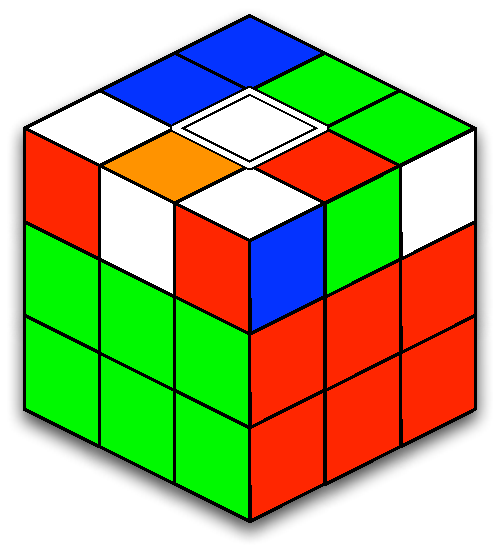
\includegraphics[width=0.28\textwidth]{input/pics/LLCPOS1}}
		\hspace{0.02\textwidth}
		\subfloat[\myCaption{The algorithm needs to be performed twice.}]{\label{fig:LLCPOS2}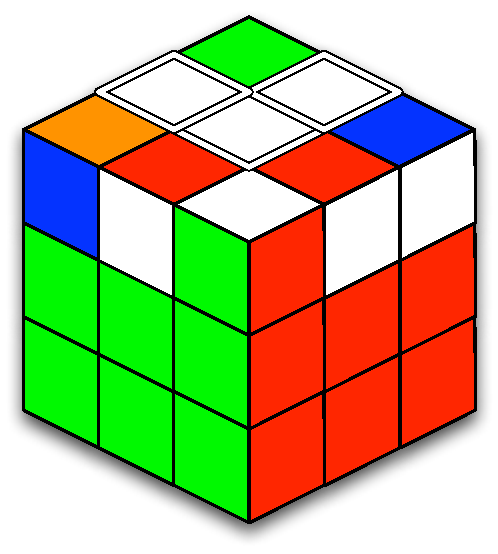
\includegraphics[width=0.28\textwidth]{input/pics/LLCPOS2}}
		\hspace{0.02\textwidth}
		\subfloat[\myCaption{The algorithm needs to be performed once.}]{\label{fig:LLCPOS3}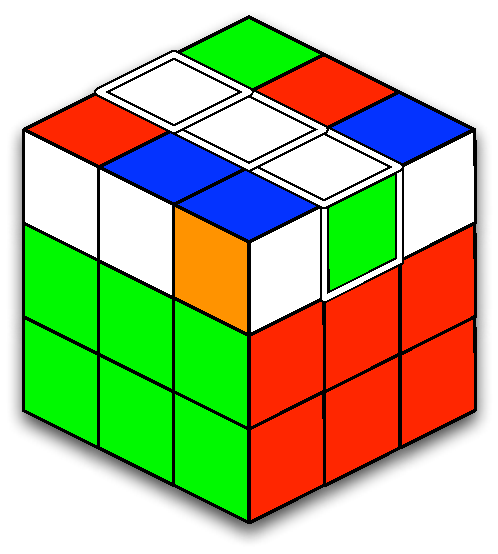
\includegraphics[width=0.28\textwidth]{input/pics/LLCPOS3}}
		\caption{\myCaption{The different top edges in the white layer can be in. }}
		\label{fig:LLCPOS}
\end{figure}


